\documentclass[conference]{IEEEtran}
\IEEEoverridecommandlockouts
% Built inside the SATNAC / IEEE conference template (v 6/27/2024).
\usepackage{cite}
\usepackage{amsmath,amssymb,amsfonts}
\usepackage{algorithmic}
\usepackage{graphicx}
\usepackage{textcomp}
\usepackage{xcolor}
\usepackage{url}
\usepackage{booktabs}
\usepackage{multirow}
\usepackage{tikz}
\usetikzlibrary{shapes, arrows, positioning, fit, backgrounds, calc}
\def\BibTeX{{\rm B\kern-.05em{\sc i\kern-.025em b}\kern-.08em
    T\kern-.1667em\lower.7ex\hbox{E}\kern-.125emX}}
\graphicspath{{figs/}{figures/}{../img/}}

\begin{document}

\title{Where to Fly the Cell Tower: Terrain-Dependent Positioning of a Nomadic
5G Node Serving Ground Robots in Disaster Search-and-Rescue}

\author{
\IEEEauthorblockN{1\textsuperscript{st} Innocent N. Makhubela}
\IEEEauthorblockA{\textit{Dept. of Electrical Engineering} \\
\textit{University of Cape Town}\\
Cape Town, South Africa}
\and
\IEEEauthorblockN{2\textsuperscript{nd} Joyce Mwangama}
\IEEEauthorblockA{\textit{Dept. of Electrical Engineering} \\
\textit{University of Cape Town}\\
Cape Town, South Africa}
\and
\IEEEauthorblockN{3\textsuperscript{rd} Given Name Surname}% TODO: author 3
\IEEEauthorblockA{\textit{dept. name of organization} \\
\textit{name of organization}\\
City, Country}
\and
\IEEEauthorblockN{4\textsuperscript{th} Given Name Surname}% TODO: author 4
\IEEEauthorblockA{\textit{dept. name of organization} \\
\textit{name of organization}\\
City, Country}
\and
\IEEEauthorblockN{5\textsuperscript{th} Given Name Surname}% TODO: author 5
\IEEEauthorblockA{\textit{dept. name of organization} \\
\textit{name of organization}\\
City, Country}
\and
\IEEEauthorblockN{6\textsuperscript{th} Given Name Surname}% TODO: author 6
\IEEEauthorblockA{\textit{dept. name of organization} \\
\textit{name of organization}\\
City, Country}
}

\maketitle

\begin{abstract}
When an earthquake, flood, or fire destroys or overwhelms terrestrial cellular
infrastructure, the ground robots increasingly used for search and rescue lose the
very connectivity they depend on to stream sensor data out and receive commands in.
A base station carried by an uncrewed aerial vehicle, a nomadic node, can restore
service on demand, but because the node is itself mobile a responder must decide
where to fly it, and that decision interacts with the terrain the robots operate in.
This paper studies that decision empirically. We build a protocol-in-the-loop
emulation that couples a physics simulator to a real fifth-generation standalone
network stack: the three-dimensional motion of an aerial base station and two
ground-robot devices continuously drives a terrain-parameterised air-to-ground
path-loss model whose output is injected at runtime into a live radio access network
and core, over which genuine bulk-upload, video, and command traffic are measured in
both directions across the emulated air interface. We instantiate five terrains,
open field, urban, forest, hills, and an enterable building, each sharing one
obstacle geometry between the rendered world and the radio channel, and run each as
a six-hour trial split into a static-node phase and a roaming-node phase while both
robots patrol. We find that the effect of node mobility on connectivity is strongly
terrain-dependent and changes sign with how pervasively the terrain blocks the link:
roaming rescues a weak device in line of sight, is neutral under localised building
shadowing, and degrades connectivity as blockage becomes pervasive, while deep
building penetration is effectively uncoverable at this link budget. We re-analyse
the logged data to derive four operational metrics for responders, and we release
the testbed, the automation, and the dataset.
\end{abstract}

\begin{IEEEkeywords}
UAV-enabled networks, non-terrestrial networks, nomadic base station, aerial base
station, 5G NR, air-to-ground channel, propagation, disaster response, search and
rescue, protocol-in-the-loop emulation, OpenAirInterface.
\end{IEEEkeywords}

\section{Introduction}

\subsection{The Disaster-Connectivity Problem}
Modern disaster response is increasingly robotic. Ground robots enter collapsed
buildings, rubble fields, flood zones, and wildfire margins that are too dangerous
for responders, streaming video and sensor data to a command post and receiving
navigation waypoints and safety-critical commands in return. This mission is built on
an implicit assumption: that a network is there to carry the traffic. In exactly the
scenarios where robots are most valuable, that assumption fails. Earthquakes and
floods topple or submerge cell sites; fires burn fibre backhaul; a surge of civilian
traffic congests whatever survives. The connectivity a rescue team depends on is cut
precisely when it is needed most, and a robot that cannot phone home is blind to its
operator and deaf to a stop command.

\subsection{UAV-Mounted Nomadic Nodes as a Response}
A base station carried aloft by an uncrewed aerial vehicle (UAV), a \emph{nomadic
node}, is a direct answer: it can be flown to the incident and provide an on-demand
aerial cell over the search area~\cite{zeng2016wireless, naqvi2018drone,
merwaday2016improved}. Its appeal for public safety is well argued---rapid
deployment, no dependence on surviving ground infrastructure, and a vantage point
that tends toward line of sight~\cite{mozaffari2019tutorial}. The concept and its
analytic air-to-ground (A2G) channel models are mature~\cite{alhourani2014optimal,
3gpp36777}.

\subsection{The Positioning Question}
Because the node is airborne and \emph{mobile}, a mission planner faces a decision a
fixed tower never poses: as robots spread through the search area, should the node
\emph{hover} at a vantage point or \emph{roam} to follow them, and at what altitude
and horizontal offset? The naive intuition---follow the robots---is not obviously
right, because the robots operate \emph{in terrain}. Buildings cast radio shadows;
tree canopies attenuate in proportion to the foliage path length; hills diffract;
walls impose penetration loss. Each mechanism loads the A2G channel differently, and
moving the node changes the \emph{propagation path} through that terrain, sometimes
clearing an obstacle and sometimes introducing one. Whether mobility helps or hurts
should therefore depend on the terrain, and the size and even the sign of that effect
is what a responder needs to know before deciding where to fly.

\subsection{Why Simulation, and What It Validates}
Answering this with fidelity is difficult. Closed-form analysis and packet-level
simulation abstract away the very mechanisms whose behaviour we want to observe: the
scheduler's reaction to changing signal quality, hybrid-ARQ retransmission under
fading, modulation-and-coding adaptation, and the radio-link-failure (RLF) and
re-establishment state machine. A live field trial with a real UAV, across five
controlled terrains for many hours each, is expensive, weather-bound, and hard to
repeat. We take a middle path: a \emph{protocol-in-the-loop} emulation that runs an
unmodified fifth-generation (5G) standalone stack and drives it with
physics-simulated robot and UAV motion through a terrain-consistent A2G channel. This
validates the \emph{mechanism and the operational rules}---how a complete protocol
stack reports connectivity as geometry and terrain change---rather than absolute
capacity, and it does so reproducibly.

\subsection{Contributions}
This paper makes four contributions.
\begin{itemize}
\item A mobility- and terrain-coupled emulation architecture
(Sections~\ref{sec:pil}--\ref{sec:channel}): the full software stack, its
inter-component communication, the geometry-to-signal pipeline, and a
terrain-parameterised A2G channel whose non-line-of-sight (NLoS) excess is derived and
evaluated on the same obstacle geometry the physics world renders.
\item A controlled hover-versus-roam study across five terrains
(Section~\ref{sec:results}), each a six-hour trial reporting both devices'
throughput, latency, coverage, and outage, establishing that the sign of the mobility
effect flips with the pervasiveness of terrain blockage.
\item Four operational metrics for disaster response, re-analysed from the logged
data (Section~\ref{sec:results}\,J): time-to-first-outage, a minimum-viable-position
rule, a governor-mediated recovery time (reported with an explicit
granularity caveat), and a per-terrain hover-versus-roam decision rule.
\item A propagation-aware coverage governor (Section~\ref{sec:gov}) that keeps robots
connected in NLoS by reacting to \emph{measured} path loss, positioned as the
rule-based baseline for a future learned controller, together with the emulation
correctness safeguards that make single-host measurement honest.
\end{itemize}
By instantiating five terrains under one instrument, we ask whether a single
positioning rule can serve a disaster responder, and find that it cannot: the right
choice of where to fly the node depends on the terrain.

\section{Related Work}
\label{sec:related}

\subsection{UAV-Enabled Networks and A2G Channel Models}
Al-Hourani \emph{et al.}~\cite{alhourani2014optimal} derived the widely used
elevation-angle model in which the probability of a line-of-sight link to a
low-altitude platform is a sigmoid of the elevation angle, and showed that an optimal
altitude balances free-space loss against the excess loss of shallow-angle links; our
channel core adopts this formulation. The tutorial of Zeng
\emph{et al.}~\cite{zeng2016wireless} and its 5G-and-beyond
follow-up~\cite{zeng2019accessing}, and the survey of Mozaffari
\emph{et al.}~\cite{mozaffari2019tutorial}, catalogue UAV placement, trajectory, and
energy trade-offs, but are predominantly analytic or system-level. 3GPP characterised
aerial channels and interference for cellular UAV support~\cite{3gpp36777} and
specified the general A2G and outdoor-to-indoor channel families~\cite{3gpp38901}.

\subsection{Terrain-Specific Propagation Models}
Terrain excess loss has long-standing empirical models we reuse verbatim. Weissberger's
modified exponential-decay model~\cite{weissberger1982} gives foliage attenuation as a
function of the depth of canopy a ray traverses; the ITU-R knife-edge
recommendation~\cite{ituP526} gives single-obstacle diffraction loss as a function of
the Fresnel-Kirchhoff parameter; and 3GPP TR~38.901~\cite{3gpp38901} specifies
outdoor-to-indoor penetration as a wall term plus a depth-dependent term. These are
normally used in isolation; a contribution here is coupling all four to one live stack
under a common testbed.

\subsection{UAV-Assisted Disaster and Public-Safety Communications}
Naqvi \emph{et al.}~\cite{naqvi2018drone} argue drone-aided communication as a key
enabler for resilient public-safety networks, restoring connectivity in disaster
regions and offloading congested cells. Merwaday and Guvenc~\cite{merwaday2016improved}
quantify the throughput and coverage gains of adding aerial base stations when
terrestrial infrastructure is damaged. This body of work motivates the deployment but
evaluates it under statistical channels; we complement it with protocol-stack
measurement across distinct terrains.

\subsection{Multi-Robot Networking for Search and Rescue}
On the robotics side, Queralta \emph{et al.}~\cite{queralta2020collaborative} survey
collaborative multi-robot search and rescue and note communication as a recurring
bottleneck, while connectivity-aware coordination
work~\cite{queralta2020collaborative} keeps robot teams within range of one another or
a base. That literature typically assumes a disc- or exponential-range communication
model; we instead measure, end-to-end on a real stack, how the \emph{base itself}
should move given roaming robots, with a channel shaped by real terrain rather than a
range disc.

\subsection{Gap This Paper Addresses}
To our knowledge, the specific combination---physics-simulated multi-robot mobility
continuously modulating a live 5G standalone stack that carries measured bidirectional
application traffic, parameterised across five terrains, and framed as a
hover-versus-roam positioning question for disaster response---has not previously been
characterised. We fill that gap and translate the result into operational rules.

\section{The Testbed Platform}
\label{sec:program}
The results here are produced on \texttt{sar\_sim}, an open testbed that couples the
Gazebo physics simulator to an OpenAirInterface (OAI) 5G standalone radio access
network (RAN) and an Open5GS core through a real-time A2G channel bridge, with each
device's data path isolated in a Linux network namespace so that traffic in both
directions genuinely crosses the emulated air interface (Section~\ref{sec:arch}). The
platform is deliberately terrain-agnostic: a world is authored once and its obstacle
geometry is shared between what Gazebo renders and what the channel model evaluates,
so five distinct terrains can be studied under one instrument with everything else
held fixed. Against that fixed platform we vary only the terrain, asking not about
node altitude alone but about the full hover-versus-roam positioning decision, and we
find that terrain can reverse the naive follow-the-robots intuition.

\section{Why Protocol-in-the-Loop Emulation}
\label{sec:pil}

\subsection{Analysis vs. Simulation vs. Emulation}
Three methods are available for studying A2G links: closed-form analysis,
packet-level simulation, and protocol-in-the-loop emulation with a real stack.
Analysis and simulation scale but abstract away the MAC scheduler, hybrid-ARQ, link
adaptation, and the RLF state machine---exactly the behaviours that turn a change in
geometry into a change in user-visible throughput, latency, and outage. Because our
question is precisely how those behaviours manifest as the node moves through terrain,
we run the actual software and inject only the physical-layer channel, trading scale
(one cell, two devices) for fidelity.

\subsection{Why OpenAirInterface}
OAI is a real, standards-compliant 5G New Radio standalone implementation, so its
scheduler, hybrid-ARQ, link adaptation, and RLF handling are genuine, not modelled.
Its \texttt{rfsimulator} backend replaces the radio front-end with a software channel
between the base and device in-phase/quadrature streams, and, decisively, exposes a
runtime channel-model interface through which per-link path loss can be set live---the
hook our mobility coupling requires. Alternatives were considered: srsRAN is likewise
open but its channel emulation is less amenable to the live per-link injection we
need, and pure simulators lack the real protocol implementation that is the point.

\subsection{Why Gazebo, Open5GS, and Supporting Tools}
Gazebo~\cite{koenig2004gazebo} provides rigid-body physics, a publish-subscribe transport for ground-truth
poses, and standard robot models. Open5GS~\cite{open5gs} supplies a production-grade 5G core so that
device attach and session establishment are genuine signalling procedures. Linux
network namespaces provide the traffic-path isolation that makes bidirectional
measurement honest, and \texttt{iperf3} and \texttt{ping} generate and measure the
flows.

\section{System Architecture}
\label{sec:arch}

\subsection{Control Loops and Data Flow}
The testbed runs three concurrent control loops on one host
(Fig.~\ref{fig:arch}); Fig.~\ref{fig:world} shows a rendered instance. The
\emph{channel loop} (2 Hz) reads poses, computes terrain-aware A2G path loss, and
injects it into the live RAN. The \emph{traffic loop} (about one cycle per robot every
15--20 s) exercises and measures each link. The \emph{mobility loop} flies the UAV and
drives the robots.

\begin{figure}[t]
\centering
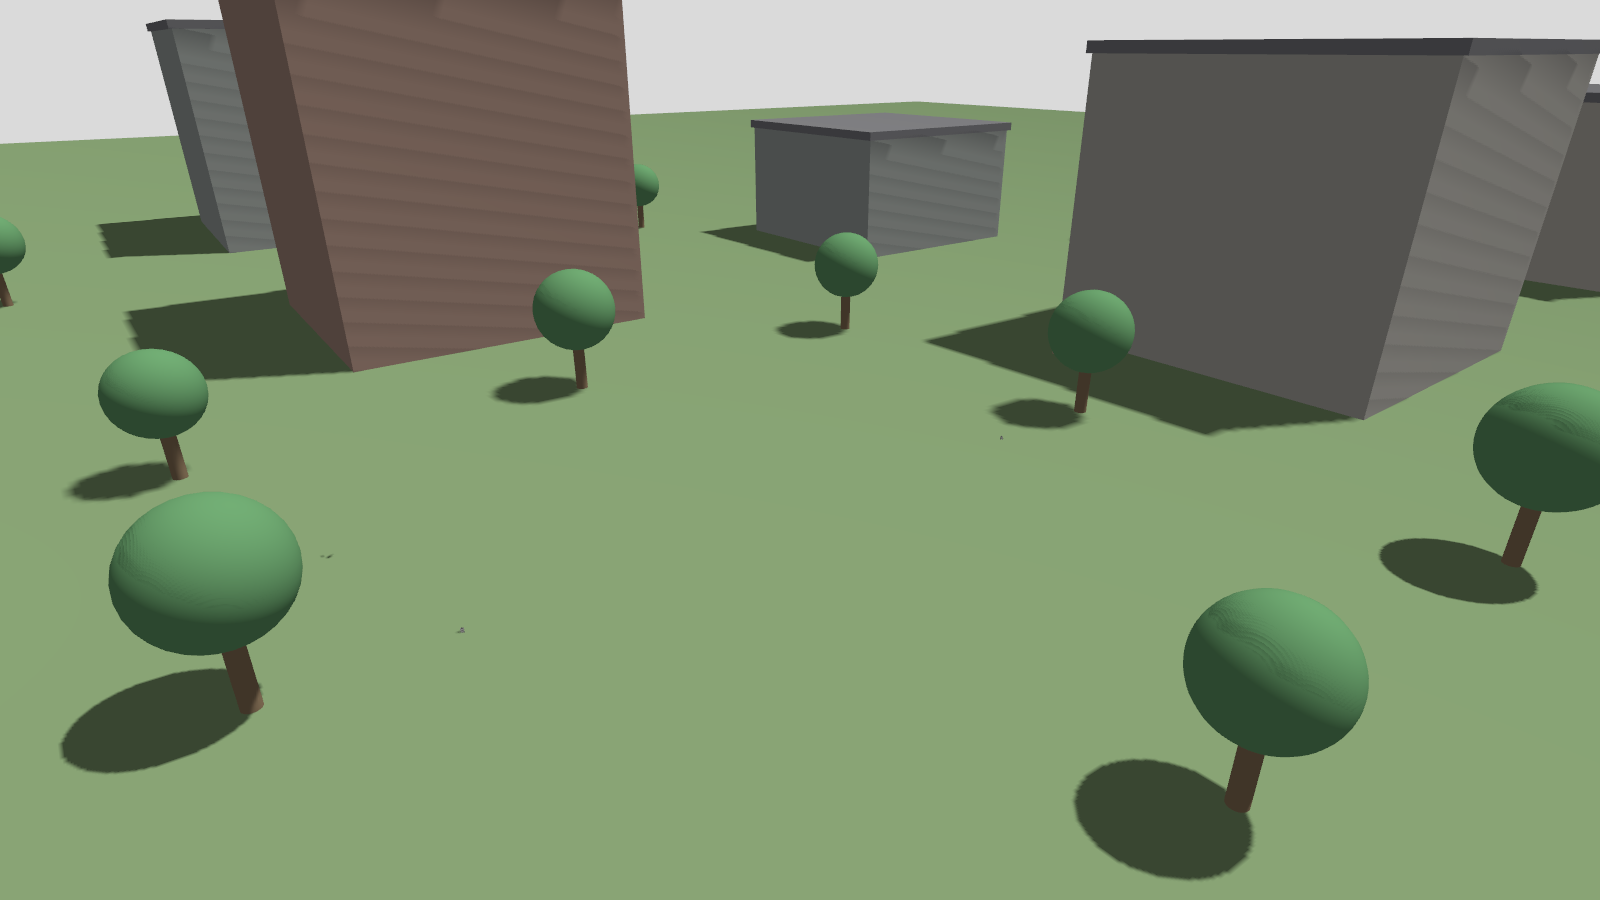
\includegraphics[width=0.94\columnwidth]{gazebo_scene.png}
\caption{A rendered terrain instance (urban). The x500 UAV carries the base station;
two ground robots are the devices. The same building footprints seen here are imported
by the channel bridge, so the radio shadowing matches the visible scene.}
\label{fig:world}
\end{figure}

\begin{figure}[t]
\centering
\begin{tikzpicture}[
  font=\scriptsize, node distance=0.45cm,
  box/.style={rectangle, draw, rounded corners, align=center, inner sep=3pt,
              fill=blue!5, minimum height=0.66cm},
  core/.style={rectangle, draw, rounded corners, align=center, inner sep=3pt,
               fill=green!8, minimum height=0.66cm},
  chip/.style={rectangle, draw, rounded corners, align=center, inner sep=2pt,
               fill=black!4, font=\tiny, minimum height=0.5cm},
  ar/.style={-latex, thick, blue!55!black},
  lbl/.style={font=\tiny\itshape, text=black!60}]
\node[box, text width=8cm] (gz) {\textbf{PHYSICS + TERRAIN --- Gazebo}\\[2pt]
  \begin{tikzpicture}[baseline]
   \node[chip,text width=1.9cm](u){sar\_uav (x500)\\\emph{carries gNB}};
   \node[chip,text width=2.0cm,right=0.22cm of u](a){robot $\alpha$\\device};
   \node[chip,text width=2.0cm,right=0.22cm of a](b){robot $\beta$\\device};
  \end{tikzpicture}};
\node[box, text width=8cm, below=0.8cm of gz] (br)
  {\textbf{CHANNEL BRIDGE --- Python}\\[1pt]
   geometry $\rightarrow$ A2G loss $L_0$ + terrain excess $\Delta_{\mathrm{env}}$
   $\rightarrow$ attenuation $A$};
\node[box, text width=4.5cm, below=0.8cm of br.south west, anchor=north west] (ran)
  {\textbf{5G RAN --- OpenAirInterface}\\[1pt] rfsimulator + channelmod\\ n78, 106 PRB};
\node[core, text width=2.9cm, right=0.3cm of ran] (cn)
  {\textbf{5G CORE --- Open5GS}\\ AMF/SMF/UPF\\ +MongoDB};
\node[box, text width=8cm, below=0.8cm of ran.south west, anchor=north west] (ns)
  {\textbf{PER-ROBOT NETWORK NAMESPACES} --- force DL/UL over the air};
\node[box, text width=8cm, below=0.6cm of ns] (tr)
  {\textbf{TRAFFIC \& MEASUREMENT} --- iperf3, ping $\rightarrow$ CSV $\rightarrow$ analysis};
\draw[ar] (gz) -- node[lbl,right]{pose/info, $\sim$10 Hz} (br);
\draw[ar] (br.south) -- ++(0,-0.4) -| node[lbl,pos=0.25,right]{channelmod, gain $=-A$, 2 Hz} (ran.north);
\draw[ar,<->] (ran) -- node[lbl,above]{N2/N3} (cn);
\draw[ar] (ran) -- node[lbl,right]{UE TUN} (ns);
\draw[ar] (ns) -- node[lbl,right]{TCP/UDP/ICMP over the air} (tr);
\end{tikzpicture}
\caption{Testbed architecture. The channel loop closes the coupling between physical
motion in terrain and radio conditions; user traffic is measured over the emulated air
interface after namespace isolation.}
\label{fig:arch}
\end{figure}

\subsection{Component Communication}
Gazebo publishes ground-truth poses on a transport topic at about 10 Hz; the bridge
subscribes and tracks the UAV and both robots, and returns velocity commands to drive
the robots. Every 0.5 s the bridge evaluates the channel (Section~\ref{sec:channel})
and writes per-link attenuation to the RAN over its control interface, with a
start-up read-back verifying each write. The \texttt{rfsimulator} carries the
base-device sample streams and applies the injected channel; the base connects to the
core over the standard N2 and N3 interfaces, and device attach performs genuine
registration and session establishment authenticated against a subscriber database.
Each device terminates in a host tunnel interface that is moved into a per-robot
namespace so downlink traffic genuinely crosses the radio (Section~\ref{sec:safe}).

\subsection{Software Stack and Versions}
Table~\ref{tab:software} lists the inventory.

\begin{table}[t]
\caption{Software stack and roles}
\label{tab:software}
\centering
\footnotesize
\begin{tabular}{@{}lll@{}}
\toprule
\textbf{Component} & \textbf{Version} & \textbf{Role} \\
\midrule
Ubuntu Linux & 22.04 LTS & Host OS (single machine) \\
Gazebo Sim (Harmonic) & 8.x & Physics; publishes 3-D poses \\
gz-transport / gz-msgs & 13 / 10 & Pub/sub bus (Python) \\
PX4 Gazebo model & x500 & UAV/gNB carrier \\
TurtleBot3 (Gazebo) & burger & Two ground-robot devices \\
OpenAirInterface & 2026.w2x & 5G NR SA RAN + rfsimulator \\
Open5GS & 2.8 & 5G core (AMF/SMF/UPF) \\
MongoDB & 6.0 & Subscriber database \\
Python & 3.10 & Bridge, mobility, analysis \\
iproute2 & 5.15 & Per-robot network namespaces \\
iperf3 & 3.16 & TCP/UDP generation and measurement \\
\bottomrule
\end{tabular}
\end{table}

\section{Geometry and the Terrain-Parameterised A2G Channel}
\label{sec:channel}

\subsection{Distances and Elevation Angle}
With the UAV at $(x_u,y_u,h_u)$ and a robot at $(x_r,y_r,h_r)$, the horizontal
distance, slant distance, and elevation angle are
\begin{align}
d_h &= \sqrt{(x_u-x_r)^2 + (y_u-y_r)^2},\\
d_{3D} &= \sqrt{d_h^2 + (h_u-h_r)^2},\\
\theta &= \arctan\!\big[(h_u-h_r)/d_h\big].
\end{align}
Two robots at equal map distance $d_h$ can experience very different links, because
the radio responds to the slant path (2) and, decisively, the elevation angle (3).

\subsection{Free-Space Loss and LoS Probability}
The free-space loss over the slant path at carrier frequency $f$ is
\begin{equation}
L_{\mathrm{FSPL}} = 20\log_{10}(d_{3D}) + 20\log_{10}(f) - 147.55,
\end{equation}
and, following~\cite{alhourani2014optimal}, the LoS probability is a sigmoid in
elevation angle, giving a base loss
\begin{align}
P_{\mathrm{LoS}}(\theta) &= \frac{1}{1 + a\,\exp[-b(\theta-a)]},\\
L_0 &= L_{\mathrm{FSPL}} + P_{\mathrm{LoS}}\,\eta_{\mathrm{LoS}}
       + (1-P_{\mathrm{LoS}})\,\eta_{\mathrm{NLoS}},
\end{align}
with $a=9.61$, $b=0.16$, $\eta_{\mathrm{LoS}}=1$ dB, $\eta_{\mathrm{NLoS}}=20$ dB.

\subsection{Terrain Excess Loss --- Worked Derivations}
The distinguishing element is an additive terrain term
$\Delta_{\mathrm{env}}$, and a possible hard LoS block, evaluated on the \emph{same}
geometry Gazebo renders. Let the base-to-device segment be $\mathbf{p}(t) =
\mathbf{p}_0 + t(\mathbf{p}_1-\mathbf{p}_0)$, $t\in[0,1]$.

\paragraph{Urban (hard blockage)}
Each building is an axis-aligned box $B=[x_0,x_1]\times[y_0,y_1]\times[z_0,z_1]$,
inflated by a margin $m$ to model grazing. Using the slab method, for axis $i$ with
$\delta_i = p_1^i-p_0^i$ the segment enters and exits the slab at
\begin{equation}
t_i^{-}=\frac{(l_i-p_0^i)}{\delta_i},\quad t_i^{+}=\frac{(u_i-p_0^i)}{\delta_i},
\end{equation}
(swapped so $t_i^{-}\!\le t_i^{+}$), with $l_i,u_i$ the inflated bounds; a segment
parallel to a slab is tested against its bounds directly. The box is struck iff
\begin{equation}
\max_i t_i^{-} \;\le\; \min_i t_i^{+}\quad\text{within } [0,1].
\end{equation}
If any building is struck, the link is NLoS: $P_{\mathrm{LoS}}\!\to\!0$ so the full
$\eta_{\mathrm{NLoS}}$ applies. Trees, by contrast, are clutter, not hard blockers.

\paragraph{Forest (Weissberger foliage)}
The foliage depth $D$ is the total length of the segment inside tree canopies, each
modelled as a sphere of centre $\mathbf{c}_j$ and radius $r_j$; the segment-sphere
overlap $[t_0,t_1]$ contributes $\lVert\mathbf{p}_1-\mathbf{p}_0\rVert\,(t_1-t_0)$,
summed over trees and capped. Weissberger's modified exponential-decay
model~\cite{weissberger1982} then gives, with $f$ in GHz and $D$ in metres,
\begin{equation}
\Delta_{\mathrm{env}}^{\mathrm{forest}} =
\begin{cases}
0.45\, f^{0.284}\, D, & 0 < D \le 14,\\[2pt]
1.33\, f^{0.284}\, D^{0.588}, & 14 < D \le 400.
\end{cases}
\end{equation}
The link is treated as NLoS once $D$ exceeds a small threshold (2 m), so foliage adds
both graded loss and a loss of the LoS bonus.

\paragraph{Hills (knife-edge diffraction)}
Each hill that intrudes into the path is a single knife edge whose top stands a height
$h$ above the straight base-device line. With $d_1,d_2$ the distances from the two
endpoints to the edge and $\lambda$ the wavelength, the Fresnel-Kirchhoff parameter is
\begin{equation}
v = h\sqrt{\frac{2}{\lambda}\!\left(\frac{1}{d_1}+\frac{1}{d_2}\right)},
\end{equation}
and the ITU-R single-edge diffraction loss~\cite{ituP526} is
\begin{equation}
J(v) =
\begin{cases}
0, & v \le -0.78,\\[2pt]
6.9 + 20\log_{10}\!\big(\sqrt{(v-0.1)^2+1} + v - 0.1\big), & v > -0.78.
\end{cases}
\end{equation}
We take $\Delta_{\mathrm{env}}^{\mathrm{hills}}=\max_j J(v_j)$ over intruding hills
(worst edge dominates), capped, and treat the link as NLoS once the loss exceeds a
threshold.

\paragraph{Indoor (3GPP outdoor-to-indoor)}
When the device lies inside the building footprint, a 3GPP-style
term~\cite{3gpp38901} applies a fixed wall penetration $L_{\mathrm{tw}}$ plus a
per-metre depth loss over the distance $d_{\mathrm{in}}$ the device sits inside:
\begin{equation}
\Delta_{\mathrm{env}}^{\mathrm{indoor}} = L_{\mathrm{tw}} + \kappa\, d_{\mathrm{in}},
\end{equation}
with $L_{\mathrm{tw}}=9$ dB, $\kappa=0.5$ dB/m, capped at 40 dB, and the interior
treated as deterministic NLoS. Outside the footprint the open-field model (5)--(6)
applies.

\subsection{Injection, Clipping, and Applied Gain}
The total loss is $L = L_0 + \Delta_{\mathrm{env}} + X_\sigma$, where $X_\sigma$ is
correlated log-normal shadow fading (larger variance under NLoS, decorrelated over
distance moved). The bridge references $L$ to $L_{\mathrm{ref}}=L_0(50\,\text{m},
30\,\text{m})$, adds a per-link baseline $L_{\mathrm{base}}$ (8 dB for $\alpha$'s
uplink, 13 dB for the weaker $\beta$), and clips:
\begin{equation}
A = \mathrm{clip}\big(L_{\mathrm{base}} + (L - L_{\mathrm{ref}}),\,0,\,45\big)\ \text{dB}.
\end{equation}
Because the RAN applies its channel field as a linear \emph{gain}
(Section~\ref{sec:safe}), the value written is $-A$, scaling each sample by
$10^{-A/20}$, a true attenuation.

\subsection{Channel Validation Against the Analytic Model}
The attenuation the RAN actually applied tracks the per-sample model prediction to
within about 1.2 dB mean absolute error, and independently the device-reported
reference signal received power falls monotonically with injected loss---an external
corroboration, since it is measured by the modem, not by us. The per-terrain
model/injected/measured agreement is shown directly in Fig.~\ref{fig:ploss}, so the
behaviour reported below is a consequence of the intended physics, not an artifact.

\section{Traffic Model and Performance Metrics}
\label{sec:metrics}

\subsection{Traffic Types}
Each cycle exercises a device with three traffic types mirroring search-and-rescue
use. \emph{Bulk upload} is a short \texttt{iperf3} TCP transfer from robot to base,
modelling a sensor dump; goodput reflects reliable-transport capacity. \emph{Video}
is a fixed 8 Mbit/s uplink stream modelling a live camera; delivered rate, loss, and
jitter reflect stream quality. \emph{Command and control} (C2) is a short sequence of
small pings from base to robot, emulating waypoints and emergency-stop; its
round-trip time and loss measure \emph{controllability}, not bandwidth.

\subsection{Standard Metrics}
We record device-reported reference signal received power and signal-to-interference-plus-noise
ratio, uplink round-trip time, packet delivery ratio, and, per traffic type, goodput,
loss, and jitter. We define \emph{C2 availability} as the fraction of samples with less
than total C2 loss, \emph{outage probability} as the fraction in total loss, and
inter-device Jain fairness over per-device mean goodput. All metrics are reported per
device ($\alpha$ stronger, $\beta$ weaker).

\subsection{New Operational Metrics for Disaster Response}
Beyond the standard set we derive four responder-facing metrics from the same logs,
defined and reported in Section~\ref{sec:results}\,J: (i) \emph{time-to-first-outage},
the safe window from link-up to first C2 loss; (ii) \emph{minimum viable position},
the largest device range sustaining at least 90\% C2 availability for the weaker
device; (iii) \emph{connectivity recovery time}, how long a dropped device takes to
return; and (iv) a \emph{hover-versus-roam decision rule} per terrain.

\section{Mobility and Propagation-Aware Coverage Governance}
\label{sec:gov}

\subsection{Naive Geometric Safe-Radius Governor and Why It Fails in NLoS}
Robots drive by differential-drive velocity commands at 1 m/s along randomised
headings. To keep them from being stranded, a governor confines each robot. A naive
governor inverts the open-field model for a \emph{geometric safe radius}
\begin{equation}
\label{eq:rsafe}
R_{\mathrm{safe}}(h)=\max\{\,d_h : L_{\mathrm{base},\beta}+[L_0(d_h,h)-L_{\mathrm{ref}}]
\le A_{\mathrm{safe}}\,\},
\end{equation}
with $A_{\mathrm{safe}}=30$ dB. This \emph{fails} in NLoS: a robot can sit well inside
$R_{\mathrm{safe}}$ yet be blocked by a building or canopy at loss near the cliff,
because the distance rule is blind to obstacles. Once such a device declares RLF, and
because a device cannot complete cell re-synchronisation while buried in deep NLoS,
restarting it fails to re-attach and the recovery loops indefinitely.

\subsection{The Propagation-Aware Governor}
We therefore make the governor react to \emph{measured} path loss. When a device's
loss is elevated it is steered toward the base ground track, raising the elevation
angle and reducing NLoS depth; if loss stays near the cliff the robot is relocated to
a small radius from the base before it dies. Indoors, where the robot must occupy the
building, it instead retreats toward the door (reducing penetration depth) and
re-enters on recovery. This prevention-first design converts an unrecoverable cascade
into rare, short outages.

\subsection{Governor as a Baseline for Future AI-Assisted Control}
The governor is a hand-tuned, threshold-based controller. It is deliberately simple,
and it is best read as a \emph{baseline}: the labelled corpus it produces---path loss,
signal quality, block-error and hybrid-ARQ trends, and outage labels, all tied to
geometry and terrain---is exactly the substrate a learned or reinforcement-learning
controller would train on to place the node and route the robots. We make no learned-control
claim in this paper; Section~\ref{sec:conclusion} sketches that direction honestly as
future work.

\section{Emulation Correctness Safeguards}
\label{sec:safe}
Building an honest single-host testbed surfaced three failure modes that produced
\emph{plausible but wrong} data; all reported results were collected only after all
three were fixed.

\subsection{The Channel Field Is a Gain, Not a Loss}
The RAN's channel field is applied as a linear gain ($10^{x/20}$): positive values
\emph{amplify} until sample clipping, so a positive ``loss'' produced a link that
degraded only through clipping and a received power that \emph{rose} with distance. We
keep $A$ positive and negate once at injection (14).

\subsection{Single-Host Traffic Bypasses the Radio}
With host-local device addresses, base-to-robot traffic went over loopback (a
``downlink'' test read gigabits per second while the base scheduled a fraction of a
megabit). Moving each tunnel into a per-robot namespace forces the air path in both
directions.

\subsection{Single-Client Control Port Silently Drops Writes}
The RAN control port accepts one client; a second connection sat unaccepted in the
backlog, silently discarding one device's channel updates and imitating a weaker
device. A shared connection per port with a start-up read-back refuses to run unless
every baseline verifies.

\section{Experimental Setup}
\label{sec:setup}

\subsection{Terrain Instantiation and Shared Geometry}
Five terrains are instantiated: open field, urban (building footprints), forest (tree
canopies), hills (a height field), and an enterable building. Each terrain authors its
obstacle geometry once; the same geometry drives both the Gazebo render and the
channel excess of Section~\ref{sec:channel}, so shadowing is consistent with the
visible scene by construction.

\subsection{Trial Structure}
Each terrain runs a single six-hour trial in two phases: \emph{phase~1} (0--3 h) with
the node hovering statically, and \emph{phase~2} (3--6 h) with the node performing a
continuous three-dimensional random walk over a bounded box while never dwelling. Both
robots free-patrol throughout, so the only variable between phases is node mobility. A
single physical stack serves only one trial (two concurrent trials share the same
robots and corrupt each other, so trials are serialised under an exclusive lock).
Clean trials comprise 733, 721, 482, and 974 samples for open field, urban, forest,
and hills; the indoor trial is reported separately as a coverage limit.

\subsection{RAN and Core Configuration}
The base operates in band n78 at 3.32 GHz, 40 MHz, 30 kHz subcarrier spacing, 106
resource blocks, connected to Open5GS over N2/N3. Exploratory runs collected while the
safeguards of Section~\ref{sec:safe} were latent are excluded from every number.

\section{Results}
\label{sec:results}

\subsection{Propagation and Coverage Across Terrains}
Fig.~\ref{fig:ploss} plots path loss against base-device slant distance per terrain,
overlaying the analytic A2G model, the value actually injected into the RAN, and the
value the device measured from its reference-signal received power. Two things stand
out. First, the injected and measured curves track one another closely in every
terrain, an end-to-end validation that the device experiences the channel we intend
(injected-versus-model agreement about 1.2 dB mean absolute error). Second,
the terrain shapes the curve: open field and hills sit low (shallow, LoS-dominated),
forest climbs steeply because a longer slant path cuts through more canopy, and urban
is intermediate with building-driven jumps. Fig.~\ref{fig:covmap} makes this spatial:
open field is a clean radial field, urban is fractured by building shadows, forest
disintegrates into thin coverage fingers, and hills form an irregular covered island.
Terrain does not merely shift coverage---it changes its \emph{shape}, so moving the
node has a terrain-specific effect. Fig.~\ref{fig:tsploss} shows the same path loss as
a time series: as the node roams (shaded), forest and hills climb toward the RLF cliff
while open field and urban stay bounded.

\begin{figure}[t]
\centering
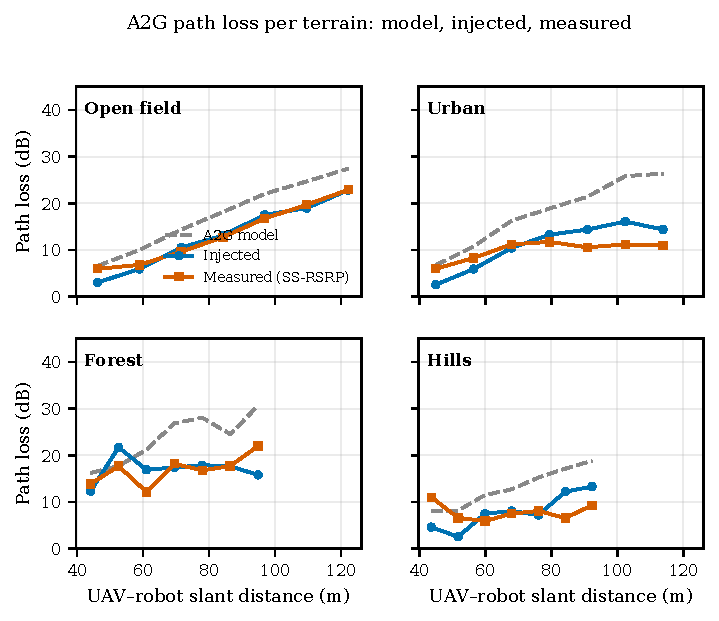
\includegraphics[width=0.86\columnwidth]{fig_ploss_model.pdf}
\caption{A2G path loss versus base-device slant distance per terrain: the analytic
model (dashed), the value injected into the RAN (blue), and the value measured by the
device from reference-signal received power (orange). Injected and measured track
closely; terrain sets the shape.}
\label{fig:ploss}
\end{figure}

\begin{figure}[t]
\centering
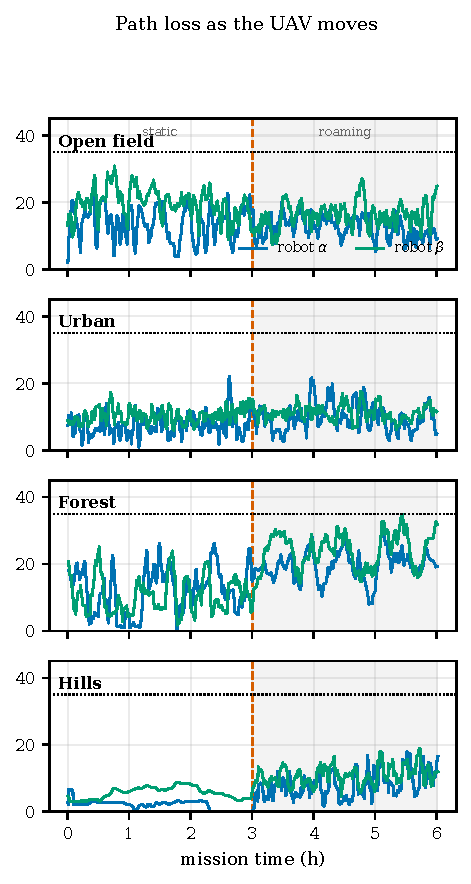
\includegraphics[width=0.66\columnwidth]{fig_ts_ploss.pdf}
\caption{Path loss over the six-hour mission as the UAV moves, per terrain, both
robots; dashed line = static-to-roaming transition (3 h), shaded = roaming, dotted =
RLF cliff. Forest and hills climb once the node roams.}
\label{fig:tsploss}
\end{figure}

\begin{figure}[t]
\centering
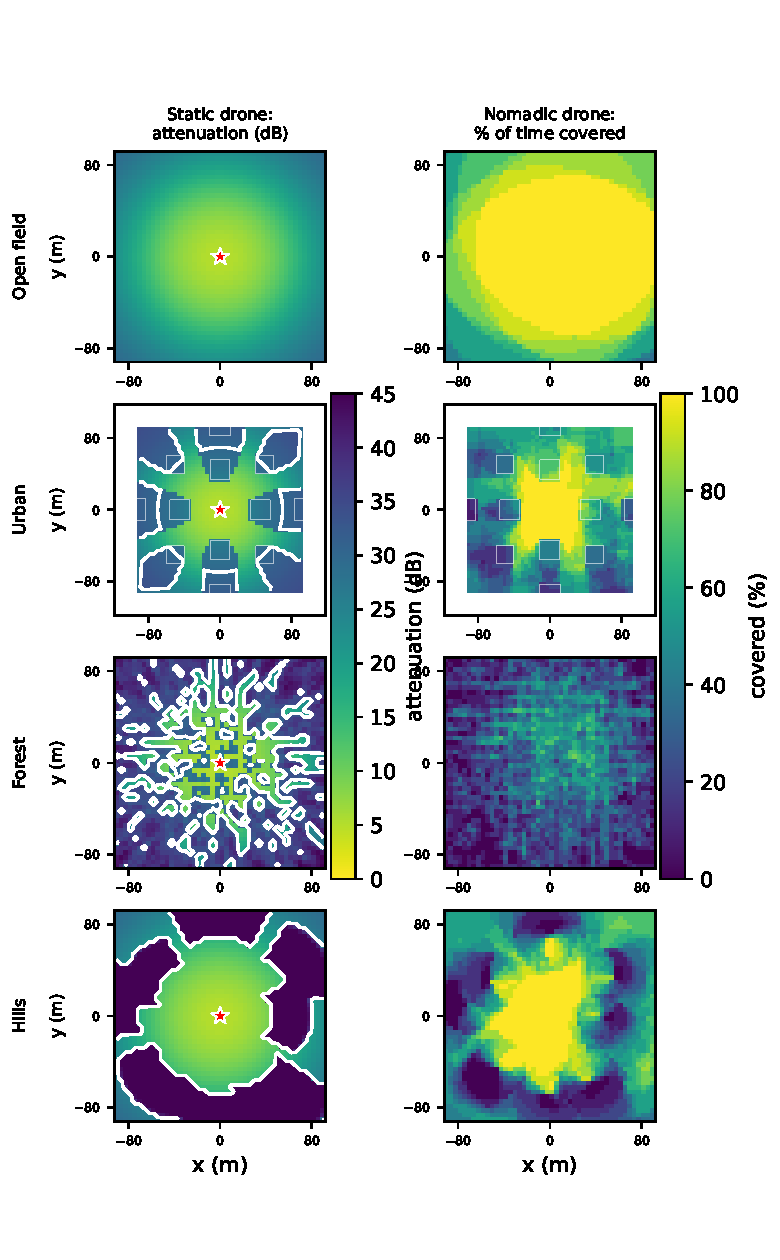
\includegraphics[width=0.72\columnwidth]{fig_coverage_map.pdf}
\caption{Coverage field over the search area (weaker device), per terrain. Left: link
attenuation for a \emph{static} node at the origin (star; white contour = usable
edge). Right: fraction of time each point is covered as a \emph{roaming} node moves.
Urban is fractured by building shadows; forest never coheres; open field spreads as
the node moves.}
\label{fig:covmap}
\end{figure}

\subsection{Watching the Drone Move}
Fig.~\ref{fig:tsc2} shows the raw phenomenon: both devices' C2 connectivity over the
full six-hour mission, per terrain, with the static-to-roaming transition marked at
3 h (shaded = roaming). In open field the weak device $\beta$ repeatedly drops while
the node is static, then steadies once it roams. In urban both devices stay flat.
In forest both are healthy while static, then connectivity collapses the moment the
node begins roaming. Hills is a milder version.

\begin{figure}[t]
\centering
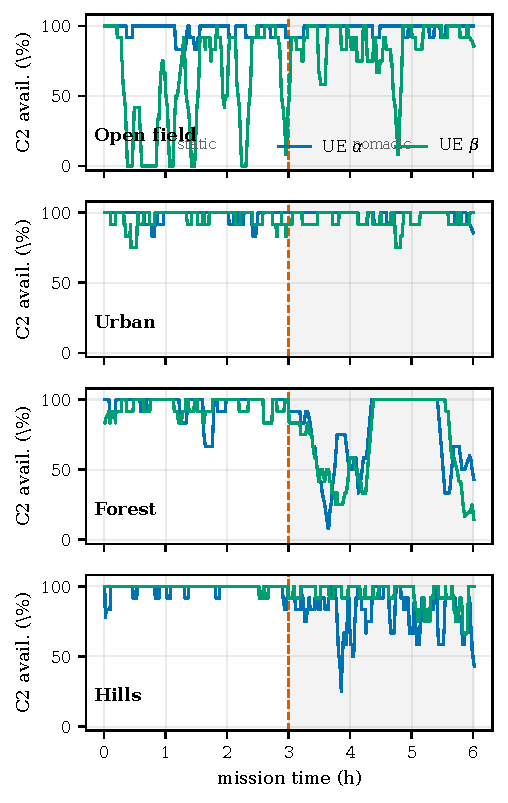
\includegraphics[width=0.8\columnwidth]{fig_ts_c2.pdf}
\caption{C2 connectivity over the six-hour mission, per terrain, both devices (rolling
availability); dashed line = static-to-roaming transition (3 h), shaded = roaming.}
\label{fig:tsc2}
\end{figure}

\subsection{Moving the Drone: The Effect Flips With Terrain}
Fig.~\ref{fig:c2} and Table~\ref{tab:main} give the central result: \textbf{the effect
of node mobility on connectivity is terrain-dependent and changes sign with the
pervasiveness of blockage.} In open field mobility \emph{helps} the weak device:
$\beta$'s C2 availability rises from 56.5\% (static) to 88.7\% (roaming), a 32
percentage-point gain, as the roaming node drifts closer and rescues a device near the
edge (mean distance falls from 91 to 75 m), while $\alpha$ stays near 98\%. In urban it
is \emph{neutral} (about 96--98\%): buildings leave LoS pockets the governor holds. In
hills and forest it \emph{hurts}, scaling with how pervasive the blockage is,
$-10.6$ points for knife-edge terrain and $-22$ points for everywhere-present foliage,
which collapses both devices to about 73--75\%.

\begin{figure}[t]
\centering
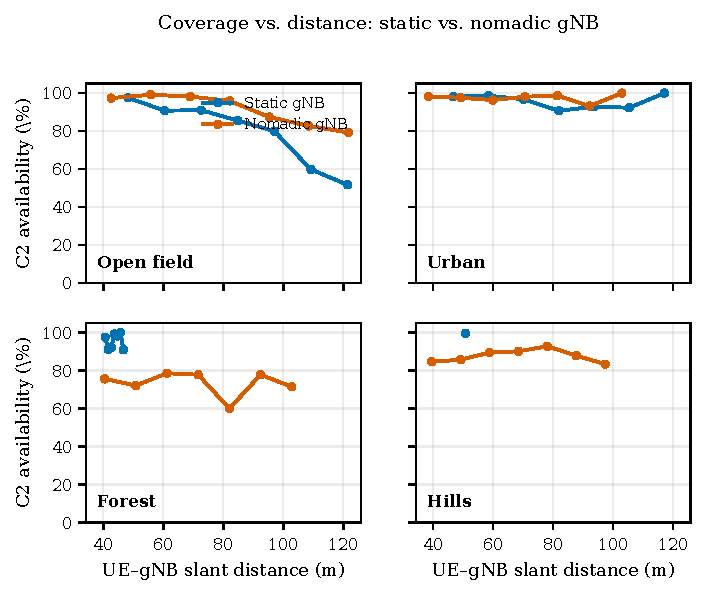
\includegraphics[width=0.86\columnwidth]{fig_coverage_distance.pdf}
\caption{C2 availability versus base-device distance, static versus roaming, per
terrain. Roaming holds coverage at range in open field; urban stays high; hills degrade
under roaming; forest cannot be sustained at range.}
\label{fig:c2}
\end{figure}

\begin{table}[t]
\centering
\caption{C2 availability and mean link metrics by terrain and node phase
(device-averaged). $\Delta$ is roaming minus static C2 (points).}
\label{tab:main}
\footnotesize
\begin{tabular}{@{}llrrrr@{}}
\toprule
Terrain & Phase & C2 (\%) & PLoss & SINR & TCP \\
        &       &         & (dB)  & (dB) & (Mb/s) \\
\midrule
\multirow{3}{*}{Open field}
 & Static  & 76.8 & 16.5 & 35.1 & 9.7  \\
 & Roaming & 93.5 & 14.2 & 38.8 & 13.1 \\
 & \multicolumn{1}{r}{$\Delta$} & \textbf{+16.7} & & & \\
\midrule
\multirow{3}{*}{Urban}
 & Static  & 97.0 & 8.8  & 43.8 & 17.6 \\
 & Roaming & 96.9 & 10.4 & 42.6 & 16.1 \\
 & \multicolumn{1}{r}{$\Delta$} & \textbf{$-$0.1} & & & \\
\midrule
\multirow{3}{*}{Hills}
 & Static  & 98.9 & 3.9  & 45.7 & 21.6 \\
 & Roaming & 88.3 & 9.3  & 44.2 & 19.4 \\
 & \multicolumn{1}{r}{$\Delta$} & \textbf{$-$10.6} & & & \\
\midrule
\multirow{3}{*}{Forest}
 & Static  & 96.2 & 10.8 & 40.9 & 15.1 \\
 & Roaming & 74.2 & 21.7 & 32.5 & 3.2  \\
 & \multicolumn{1}{r}{$\Delta$} & \textbf{$-$22.0} & & & \\
\bottomrule
\end{tabular}
\end{table}

\subsection{Mission Cost: Streaming and Control}
Connectivity translates directly into mission capability (Fig.~\ref{fig:video}). The
8 Mbit/s video feed---the operator's eyes---arrives nearly intact in open field, urban,
and hills, but in forest a roaming node drives it to 1.9 Mbit/s with over 70\% loss:
the operator goes blind exactly when the node moves. Command latency, by contrast,
holds near 37 ms median \emph{whenever the link is up}, in every terrain and phase, so
controllability fails as an \emph{availability} problem, not a latency creep.

\begin{figure}[t]
\centering
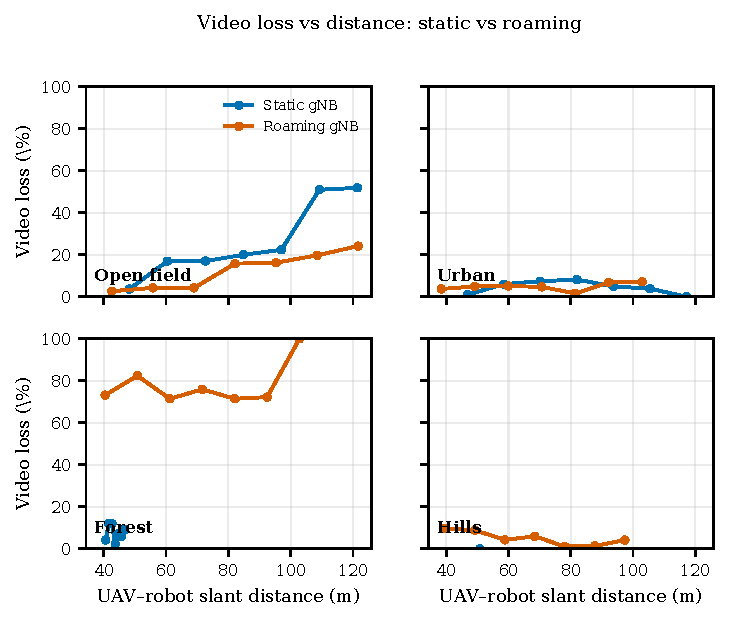
\includegraphics[width=0.86\columnwidth]{fig_video_distance.pdf}
\caption{Video packet loss versus base-device distance, static versus roaming, per
terrain. Forest loss climbs sharply under roaming (delivered video falls to
1.9 Mbit/s); open field, urban, and hills stay low.}
\label{fig:video}
\end{figure}

\subsection{Throughput and Coverage as the UE Moves}
Fig.~\ref{fig:tputdist} plots TCP goodput against base-device distance, static versus
roaming, per terrain. In open field the static curve falls off a coverage cliff with
range while the roaming node flattens it by following the robot; in forest both curves
sit low and roaming cannot lift them. Moving the node buys range where the path is
clear and buys nothing where it is blocked.

\begin{figure}[t]
\centering
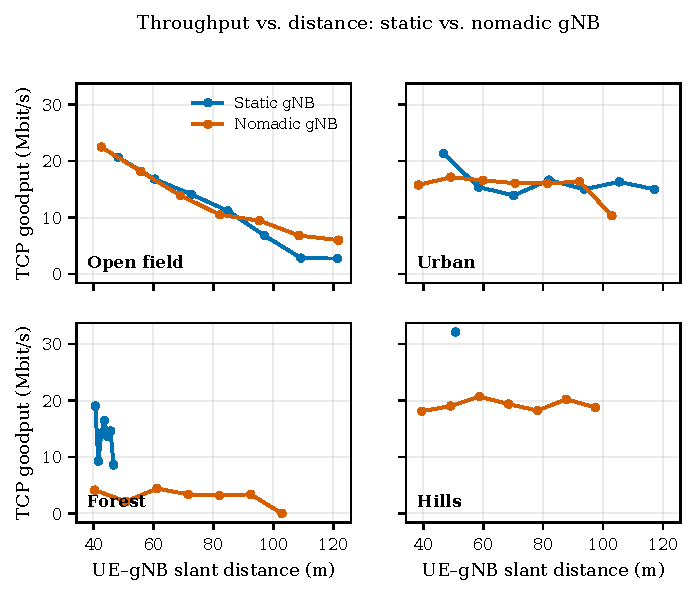
\includegraphics[width=0.78\columnwidth]{fig_tput_distance.pdf}
\caption{TCP goodput versus base-device distance, static versus roaming node, per
terrain. Roaming flattens the open-field cliff but cannot lift the blocked forest
link.}
\label{fig:tputdist}
\end{figure}

\subsection{The Real Stack Adapts}
Because we run a genuine RAN, link adaptation is observed, not modelled
(Fig.~\ref{fig:linkadapt}). As the forest-roaming channel degrades, the scheduler
backs uplink spectral efficiency down (from 4.2 to 2.7 bits/symbol) while hybrid-ARQ
holds block error near target (below 0.04\%): the protocol trades rate for reliability,
which a link-level abstraction would miss. This is the payoff of protocol-in-the-loop
emulation.

\begin{figure}[t]
\centering
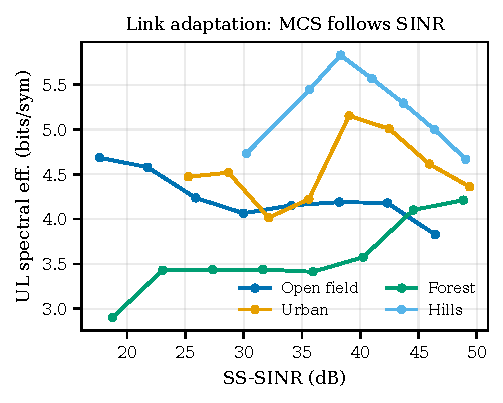
\includegraphics[width=0.8\columnwidth]{fig_linkadapt_line.pdf}
\caption{Uplink spectral efficiency versus SINR per terrain. The scheduler raises the
modulation-and-coding scheme with SINR; forest operates at low SINR and is forced to a
lower rate, while hybrid-ARQ keeps block error bounded.}
\label{fig:linkadapt}
\end{figure}

\subsection{Device Budget and the Weakest Radio}
The two devices differ only by 5 dB of baseline budget yet experience qualitatively
different networks: $\alpha$ is distance-limited while $\beta$ is budget-limited,
reaching the cliff sooner and defining the team's usable region. High Jain fairness
(about 0.97) confirms the disparity is device budget, not scheduler bias, so the remedy
is coverage margin, and node placement must be sized for the \emph{weakest} radio, in
every terrain.

\subsection{Keeping Robots Connected in NLoS}
The propagation-aware governor eliminates the RLF cascade in urban and hills (zero
failed re-attaches) and contains it in forest, where the governor intervenes 574 times
per trial, roughly once every 37 s, to keep robots out of foliage dead zones. The cost
of prevention is a more base-centred robot distribution (the concentrated roaming
coverage of Fig.~\ref{fig:covmap}); without it the cluttered terrains fail to produce
data at all.

\subsection{Indoor: A Coverage Limit}
The building terrain is qualitatively different (Fig.~\ref{fig:indoor}). The fixed
wall penetration plus the link baseline places the \emph{entire} interior near the RLF
cliff---depth barely matters---so shadow spikes trip RLF repeatedly, and each
re-attach dominates the timeline. Lowering the node to hover directly overhead (cutting
about 7 dB of A2G loss) and adding the retreat-to-door recovery removes the cascade and
keeps robots alive, but C2 availability remains only 12--18\%. A ground robot cannot
hold connectivity deep inside a building at this link budget: leaving the building is
the only recovery.

\begin{figure}[t]
\centering
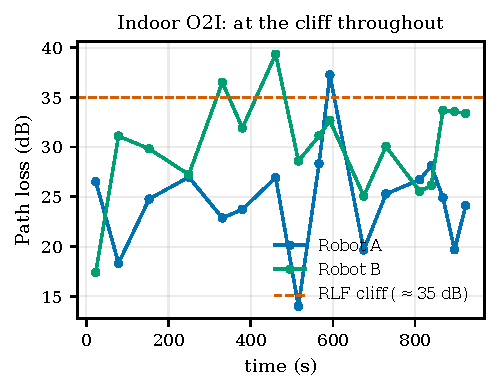
\includegraphics[width=0.78\columnwidth]{fig_indoor.pdf}
\caption{Indoor penetration path loss over time (low-hovering node). Both robots sit at
the RLF cliff throughout; the interior offers no reliably covered pocket.}
\label{fig:indoor}
\end{figure}

\subsection{Operational Metrics for Disaster Response}
We re-analyse the same logs into four responder-facing quantities
(Table~\ref{tab:ops}).

\emph{(1) Time-to-first-outage.} Measured from link-up to the first C2 loss of the
weak device, this is the ``safe window'' after a responder flies in. It is a
single-event measure and therefore noisy, but the pattern is operationally useful: in
forest, a device is already at risk within minutes, whereas in open field and hills a
static node buys a substantially longer window.

\emph{(2) Minimum viable position.} Expressed as the largest slant range at which the
weak device still holds at least 90\% C2 availability, this is a deployable
rule-of-thumb: keep the node within roughly 70 m of the weakest robot in open field,
90 m in urban, and 100 m in hills, whereas in forest no range sustains 90\% and the
node must sit almost overhead. This gives a responder a terrain-specific horizontal
bound to hold the weakest robot inside.

\emph{(3) Connectivity recovery time.} From the governor's recovery events, the mean
and 95th-percentile time from detection to a restored device are 144/199 s (open
field), 103/104 s (urban), 107/115 s (hills), and, worst by far, 207/383 s (forest)
(Fig.~\ref{fig:recovery}). \textbf{Caveat.} This is a \emph{governor-mediated} recovery
time: it is floored by the 90 s sustained-loss confirmation window and the re-attach
latency, the C2 channel is sampled only about every 25 s, and it therefore does not
measure the RAN's intrinsic radio-link re-establishment time. Reporting the true RRC
recovery time would require per-event radio-state timestamps at sub-second resolution
(available in the modem logs but not in the current per-cycle CSV), i.e.\ a logging
change or a targeted re-run; we do not approximate it from availability.

\emph{(4) Hover-versus-roam decision rule.} Restating the $\Delta$ of
Table~\ref{tab:main} as an instruction: \emph{open field, roam} (mobility helps the
weak device); \emph{urban, either} (neutral); \emph{hills and forest, hover} (mobility
hurts, most severely in forest); \emph{indoor, hover low and overhead, and expect the
deep interior to be uncoverable}.

\begin{table}[t]
\centering
\caption{Operational metrics for disaster response, per terrain (weaker device)}
\label{tab:ops}
\footnotesize
\begin{tabular}{@{}lcccc@{}}
\toprule
 & \textbf{Open} & & & \\
\textbf{Metric} & \textbf{field} & \textbf{Urban} & \textbf{Hills} & \textbf{Forest} \\
\midrule
Safe window, static (min)     & 14.8 & 7.7 & 152.7 & 2.7 \\
Viable range, $\ge$90\% (m)   & 70   & 90  & 100   & $<$overhead \\
Recovery, mean/p95 (s)        & 144/199 & 103/104 & 107/115 & 207/383 \\
Decision                      & roam & either & hover & hover \\
\bottomrule
\end{tabular}
\end{table}

\begin{figure}[t]
\centering
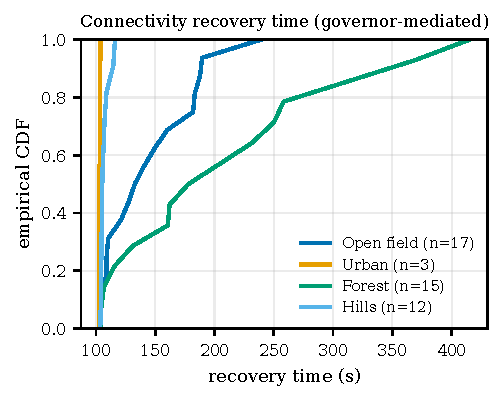
\includegraphics[width=0.8\columnwidth]{fig_recovery_cdf.pdf}
\caption{Empirical CDF of governor-mediated connectivity recovery time per terrain.
Forest has the heaviest tail; see the caveat in the text.}
\label{fig:recovery}
\end{figure}

\section{Discussion}
\label{sec:discussion}

\subsection{Why the Effect of Mobility Flips With Terrain}
Moving the node changes the \emph{propagation path}, and whether that helps depends on
how blockage is distributed. In line of sight a moving node is pure geometric benefit:
it can shorten links and rescue edge robots, so roaming helps the weak device most.
Where blockage is \emph{localised} (urban buildings), a governor can keep robots in
line-of-sight pockets and mobility washes out. Where blockage is \emph{pervasive}
(forest canopy) there is no pocket to hold: any repositioning that lengthens the ground
path lengthens the foliage path, so mobility is strictly harmful, and the damage scales
with blockage density (hills below forest). Altitude still helps by raising the
elevation angle, but in pervasive clutter the horizontal component of roaming can undo
that gain, which is why a single follow-the-robots rule fails and the decision must be
made per terrain.

\subsection{Operating Rules for SAR Deployment}
Two rules follow. First, choose hover versus roam by terrain, per
Table~\ref{tab:ops}: roam in open ground and to rescue stranded devices, hover in
foliage and rough terrain, and hover low and overhead for indoor. Second, size
coverage for the weakest radio: a few decibels of device disparity relocate the usable
edge and multiply the outage rate, so the node's position must protect $\beta$, not the
team average.

\subsection{Implications for a Learned/AI-Assisted Controller}
The terrain-dependence is precisely what makes hand-tuned control brittle and a learned
controller attractive: the right node position is a function of terrain, robot
geometry, and live link telemetry that our threshold governor only crudely
approximates. The governor and the labelled corpus it produces are the baseline and
training substrate for such a controller; we make no learned-control claim here and
develop the direction as future work.

\section{Limitations}
\label{sec:limitations}
The RAN runs over a radio-channel simulator, so absolute link budgets depend on model
constants and the configured noise floor; we therefore emphasise \emph{relative}
static-versus-roaming effects within a fixed calibration rather than absolute edges.
The coverage governor is necessary to obtain data in NLoS but alters robot
trajectories (more base-centred), so the reported effects are conditional on
prevention-based coverage keeping. We study one cell and two devices; multi-cell
handover and many-robot contention are future work. Under outage the per-sample probes
time out, so heavily degraded phases yield fewer samples, and the recovery-time metric
is governor-mediated and coarsely sampled (Section~\ref{sec:results}\,J). The indoor
result reflects one building geometry and link budget. Subject to these, the
\emph{direction} of the findings follows from geometry, link budget, and protocol-state
mechanisms that carry to physical deployments.

\section{Conclusion and Future Work}
\label{sec:conclusion}

\subsection{Summary of Findings}
We built a mobility- and terrain-coupled 5G emulation testbed for UAV-mounted nomadic
nodes serving ground robots, and used it to measure how two devices report their
connectivity as the node moves, across five terrains. The effect of node mobility is
terrain-dependent and changes sign with the pervasiveness of blockage: helpful in line
of sight, neutral under localised urban shadowing, and increasingly harmful under
diffraction and foliage, while deep indoor penetration is effectively uncoverable. We
translated the result into four operational metrics and a per-terrain hover-versus-roam
rule, and showed that connectivity in NLoS survives only under a propagation-aware
governor.

\subsection{Path Toward AI-Assisted Coverage Control}
The clear next step is to replace the threshold governor with a learned controller that
positions the node and routes robots from live telemetry and a terrain estimate,
trained and evaluated on this testbed and its dataset, with the rule-based governor as
its safety baseline.

\subsection{Multi-Cell Handover, Recovery-Time Study, and SDR Validation}
Three further directions are a multi-node handover study, a fine-grained
radio-link recovery-time measurement using per-event radio-state timestamps (addressing
the caveat above), and a software-defined-radio hardware bridge to close the
simulation-to-hardware gap.

\section*{Acknowledgment}
This work was supported by the Telkom-NRF FutureTech Programme and DIGITAfrica
(Horizon Europe). The authors thank the OpenAirInterface and Open5GS communities.
(For double-blind review, this section and the author block are anonymised.)

\footnotesize
\begin{thebibliography}{00}
\bibitem{zeng2016wireless} Y. Zeng, R. Zhang, and T. J. Lim, ``Wireless communications
with unmanned aerial vehicles: Opportunities and challenges,'' \textit{IEEE Commun.
Mag.}, vol.~54, no.~5, pp.~36--42, 2016.
\bibitem{zeng2019accessing} Y. Zeng, Q. Wu, and R. Zhang, ``Accessing from the sky: A
tutorial on UAV communications for 5G and beyond,'' \textit{Proc. IEEE}, vol.~107,
no.~12, pp.~2327--2375, 2019.
\bibitem{mozaffari2019tutorial} M. Mozaffari, W. Saad, M. Bennis, Y.-H. Nam, and
M. Debbah, ``A tutorial on UAVs for wireless networks: Applications, challenges, and
open problems,'' \textit{IEEE Commun. Surveys Tuts.}, vol.~21, no.~3, pp.~2334--2360,
2019.
\bibitem{alhourani2014optimal} A. Al-Hourani, S. Kandeepan, and S. Lardner, ``Optimal
LAP altitude for maximum coverage,'' \textit{IEEE Wireless Commun. Lett.}, vol.~3,
no.~6, pp.~569--572, 2014.
\bibitem{naqvi2018drone} S. A. R. Naqvi, S. A. Hassan, H. Pervaiz, and Q. Ni,
``Drone-aided communication as a key enabler for 5G and resilient public safety
networks,'' \textit{IEEE Commun. Mag.}, vol.~56, no.~1, pp.~36--42, 2018.
\bibitem{merwaday2016improved} A. Merwaday and I. Guvenc, ``UAV assisted heterogeneous
networks for public safety communications,'' in \textit{Proc. IEEE WCNC Workshops},
2015, pp.~329--334.
\bibitem{3gpp36777} 3GPP, ``Study on enhanced LTE support for aerial vehicles,''
TR~36.777, 2017.
\bibitem{3gpp38901} 3GPP, ``Study on channel model for frequencies from 0.5 to 100
GHz,'' TR~38.901, 2020.
\bibitem{weissberger1982} M. A. Weissberger, ``An initial critical summary of models
for predicting the attenuation of radio waves by trees,'' Electromagn. Compat. Analysis
Center, ECAC-TR-81-101, 1982.
\bibitem{ituP526} ITU-R, ``Propagation by diffraction,'' Recommendation P.526.
\bibitem{queralta2020collaborative} J. P. Queralta \textit{et al.}, ``Collaborative
multi-robot search and rescue: Planning, coordination, perception, and active vision,''
\textit{IEEE Access}, vol.~8, pp.~191617--191643, 2020.
\bibitem{nikaein2014oai} N. Nikaein \textit{et al.}, ``OpenAirInterface: A flexible
platform for 5G research,'' \textit{ACM SIGCOMM Comput. Commun. Rev.}, vol.~44, no.~5,
pp.~33--38, 2014.
\bibitem{open5gs} Open5GS, ``Open source implementation of the 5G core network,''
\url{https://open5gs.org}, accessed 2026.
\bibitem{koenig2004gazebo} N. Koenig and A. Howard, ``Design and use paradigms for
Gazebo, an open-source multi-robot simulator,'' in \textit{Proc. IEEE/RSJ IROS}, 2004,
pp.~2149--2154.
\end{thebibliography}

\end{document}
